\apendice{Esquemático Eletrônico}
\label{ap:A}

Esquemático eletrônicos dos circuitos do hardware proposto.

%Código fonte para inserir um arquivo em PDF

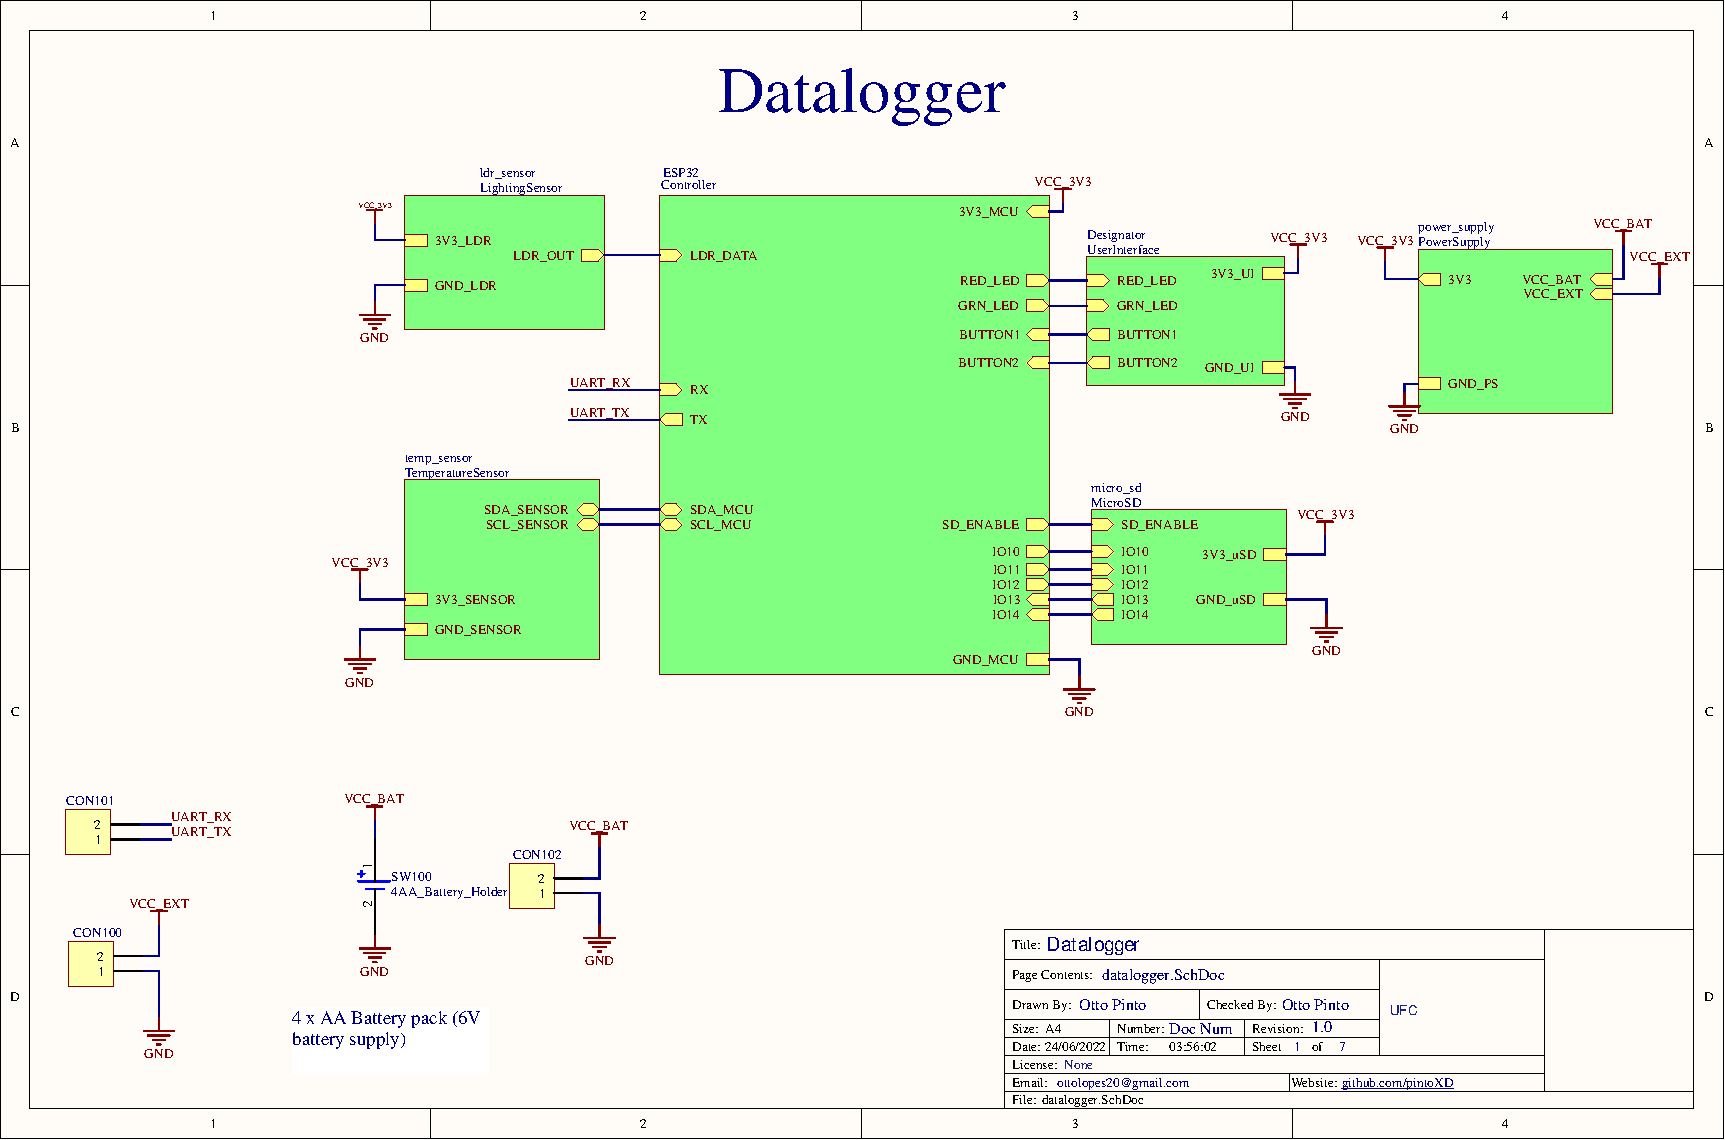
\includepdf[pages={1}, landscape=true, scale = 0.9]{3-pos-textuais/apendices/arquivos/Datalogger.PDF}

\includepdf[pages={2-7}, landscape=true, scale = 0.9]{3-pos-textuais/apendices/arquivos/Datalogger.PDF}


% Um apêndice é um documento elaborado pelo autor, diferentemente do anexo. Geralmente, se coloca como apêndice, questionários, códigos de programação, tabelas que tomariam muito espaço no meio do trabalho. Artigos, resumos ou qualquer publicação relacionada ao trabalho podem ser utilizados como apêndice.